%!TEX TS-program = xelatex

% Шаблон документа LaTeX создан в 2018 году
% Алексеем Подчезерцевым
% В качестве исходных использованы шаблоны
%     Данилом Фёдоровых (danil@fedorovykh.ru)
%        https://www.writelatex.com/coursera/latex/5.2.2
%    LaTeX-шаблон для русской кандидатской диссертации и её автореферата.
%        https://github.com/AndreyAkinshin/Russian-Phd-LaTeX-Dissertation-Template

\documentclass[a4paper,14pt]{article}


%%% Работа с русским языком
\usepackage[english,russian]{babel}   %% загружает пакет многоязыковой вёрстки
\usepackage{fontspec}      %% подготавливает загрузку шрифтов Open Type, True Type и др.
\defaultfontfeatures{Ligatures={TeX},Renderer=Basic}  %% свойства шрифтов по умолчанию
\setmainfont[Ligatures={TeX,Historic}]{Times New Roman} %% задаёт основной шрифт документа
\setsansfont{Comic Sans MS}                    %% задаёт шрифт без засечек
\setmonofont{Courier New}
\usepackage{indentfirst}
\frenchspacing

\renewcommand{\epsilon}{\ensuremath{\varepsilon}}
\renewcommand{\phi}{\ensuremath{\varphi}}
\renewcommand{\kappa}{\ensuremath{\varkappa}}
\renewcommand{\le}{\ensuremath{\leqslant}}
\renewcommand{\leq}{\ensuremath{\leqslant}}
\renewcommand{\ge}{\ensuremath{\geqslant}}
\renewcommand{\geq}{\ensuremath{\geqslant}}
\renewcommand{\emptyset}{\varnothing}

%%% Дополнительная работа с математикой
\usepackage{amsmath,amsfonts,amssymb,amsthm,mathtools} % AMS
\usepackage{icomma} % "Умная" запятая: $0,2$ --- число, $0, 2$ --- перечисление

%% Номера формул
%\mathtoolsset{showonlyrefs=true} % Показывать номера только у тех формул, на которые есть \eqref{} в тексте.
%\usepackage{leqno} % Нумерация формул слева	

%% Перенос знаков в формулах (по Львовскому)
\newcommand*{\hm}[1]{#1\nobreak\discretionary{}
	{\hbox{$\mathsurround=0pt #1$}}{}}

%%% Работа с картинками
\usepackage{graphicx}  % Для вставки рисунков
\graphicspath{{images/}}  % папки с картинками
\setlength\fboxsep{3pt} % Отступ рамки \fbox{} от рисунка
\setlength\fboxrule{1pt} % Толщина линий рамки \fbox{}
\usepackage{wrapfig} % Обтекание рисунков текстом

%%% Работа с таблицами
\usepackage{array,tabularx,tabulary,booktabs} % Дополнительная работа с таблицами
\usepackage{longtable}  % Длинные таблицы
\usepackage{multirow} % Слияние строк в таблице
\usepackage{float}% http://ctan.org/pkg/float

%%% Программирование
\usepackage{etoolbox} % логические операторы


%%% Страница
\usepackage{extsizes} % Возможность сделать 14-й шрифт
\usepackage{geometry} % Простой способ задавать поля
\geometry{top=20mm}
\geometry{bottom=20mm}
\geometry{left=20mm}
\geometry{right=10mm}
%
%\usepackage{fancyhdr} % Колонтитулы
% 	\pagestyle{fancy}
%\renewcommand{\headrulewidth}{0pt}  % Толщина линейки, отчеркивающей верхний колонтитул
% 	\lfoot{Нижний левый}
% 	\rfoot{Нижний правый}
% 	\rhead{Верхний правый}
% 	\chead{Верхний в центре}
% 	\lhead{Верхний левый}
%	\cfoot{Нижний в центре} % По умолчанию здесь номер страницы

\usepackage{setspace} % Интерлиньяж
\onehalfspacing % Интерлиньяж 1.5
%\doublespacing % Интерлиньяж 2
%\singlespacing % Интерлиньяж 1

\usepackage{lastpage} % Узнать, сколько всего страниц в документе.

\usepackage{soul} % Модификаторы начертания

\usepackage{hyperref}
\usepackage[usenames,dvipsnames,svgnames,table,rgb]{xcolor}
\hypersetup{				% Гиперссылки
	unicode=true,           % русские буквы в раздела PDF
	pdftitle={Практическая по БД},   % Заголовок
	pdfauthor={Подчезерцев Алексей},      % Автор
	pdfsubject={Создание и заполнение отношений БД фитнес-клуба},      % Тема
	pdfcreator={Подчезерцев Алексей}, % Создатель
	pdfproducer={Подчезерцев Алексей}, % Производитель
	pdfkeywords={БД} {SQL} {MySQL}, % Ключевые слова
	colorlinks=true,       	% false: ссылки в рамках; true: цветные ссылки
	linkcolor=black,          % внутренние ссылки
	citecolor=black,        % на библиографию
	filecolor=magenta,      % на файлы
	urlcolor=black           % на URL
}
\makeatletter 
\def\@biblabel#1{#1. } 
\makeatother
\usepackage{cite} % Работа с библиографией
%\usepackage[superscript]{cite} % Ссылки в верхних индексах
%\usepackage[nocompress]{cite} % 
\usepackage{csquotes} % Еще инструменты для ссылок

\usepackage{multicol} % Несколько колонок

\usepackage{tikz} % Работа с графикой
\usepackage{pgfplots}
\usepackage{pgfplotstable}

% ГОСТ заголовки
\usepackage[font=small]{caption}
%\captionsetup[table]{justification=centering, labelsep = newline} % Таблицы по правобу краю
%\captionsetup[figure]{justification=centering} % Картинки по центру


\newcommand{\tablecaption}[1]{\addtocounter{table}{1}\small \begin{flushright}\tablename \ \thetable\end{flushright}%	
\begin{center}#1\end{center}}

\newcommand{\imref}[1]{Рис.~\ref{#1}}

\usepackage{multirow}
\usepackage{spreadtab}
\newcolumntype{K}[1]{@{}>{\centering\arraybackslash}p{#1cm}@{}}


\usepackage{xparse}
\ExplSyntaxOn
\DeclareExpandableDocumentCommand{\juliandate}{ m m m }
{
	\juliandate_calc:nnnn { #1 } { #2 } { #3 } { \use:n }
}
\NewDocumentCommand{\storejuliandate}{ s m m m m }
{
	\IfBooleanTF{#1}
	{
		\juliandate_calc:nnnn { #3 } { #4 } { #5 } { \cs_set:Npx #2 }
	}
	{
		\juliandate_calc:nnnn { #3 } { #4 } { #5 } { \cs_new:Npx #2 }
	}
}
\cs_new:Npn \juliandate_calc:nnnn #1 #2 #3 #4 % #1 = day, #2 = month, #3 = year, #4 = what to do
{
	#4 
	{
		\int_eval:n
		{
			#1 +
			\int_div_truncate:nn { 153 * (#2 + 12 * \int_div_truncate:nn { 14 - #2 } { 12 } - 3) + 2 } { 5 } +
			365 * (#3 + 4800 - \int_div_truncate:nn { 14 - #2 } { 12 } ) +
			\int_div_truncate:nn { #3 + 4800 - \int_div_truncate:nn { 14 - #2 } { 12 } } { 4 } -
			\int_div_truncate:nn { #3 + 4800 - \int_div_truncate:nn { 14 - #2 } { 12 } } { 100 } + 
			\int_div_truncate:nn { #3 + 4800 - \int_div_truncate:nn { 14 - #2 } { 12 } } { 400 } -
			32045
		}
	}
}

\tl_new:N \l__juliandate_g_tl
\tl_new:N \l__juliandate_dg_tl
\tl_new:N \l__juliandate_c_tl
\tl_new:N \l__juliandate_dc_tl
\tl_new:N \l__juliandate_b_tl
\tl_new:N \l__juliandate_db_tl
\tl_new:N \l__juliandate_a_tl
\tl_new:N \l__juliandate_da_tl
\tl_new:N \l__juliandate_y_tl
\tl_new:N \l__juliandate_m_tl
\tl_new:N \l__juliandate_d_tl
\int_new:N \l_juliandate_day_int
\int_new:N \l_juliandate_month_int
\int_new:N \l_juliandate_year_int

\cs_new:Npn \__juliandate_set:nn #1 #2
{
	\tl_set:cx { l__juliandate_#1_tl } { \int_eval:n { #2 } }
}
\cs_new:Npn \__juliandate_use:n #1
{
	\tl_use:c { l__juliandate_#1_tl }
}
\cs_new_protected:Npn \juliandate_reverse:n #1
{
	\__juliandate_set:nn { g }
	{ \int_div_truncate:nn { #1 + 32044 } { 146097 } }
	\__juliandate_set:nn { dg }
	{ \int_mod:nn { #1 + 32044 } { 146097 } }
	\__juliandate_set:nn { c }
	{ \int_div_truncate:nn { ( \int_div_truncate:nn { \__juliandate_use:n { dg } } { 36524 } + 1) * 3 } { 4 } }
	\__juliandate_set:nn { dc }
	{ \__juliandate_use:n { dg } - \__juliandate_use:n { c } * 36524 }
	\__juliandate_set:nn { b }
	{ \int_div_truncate:nn { \__juliandate_use:n { dc } } { 1461 } }
	\__juliandate_set:nn { db }
	{ \int_mod:nn { \__juliandate_use:n { dc } } { 1461 } }
	\__juliandate_set:nn { a }
	{ \int_div_truncate:nn { ( \int_div_truncate:nn { \__juliandate_use:n { db } } { 365 } + 1) * 3 } { 4 } }
	\__juliandate_set:nn { da }
	{ \__juliandate_use:n { db } - \__juliandate_use:n { a } * 365 }
	\__juliandate_set:nn { y }
	{
		\__juliandate_use:n { g } * 400 + 
		\__juliandate_use:n { c } * 100 + 
		\__juliandate_use:n { b } * 4 + 
		\__juliandate_use:n { a }
	}
	\__juliandate_set:nn { m }
	{ \int_div_truncate:nn { \__juliandate_use:n { da } * 5 + 308 } { 153 } - 2 }
	\__juliandate_set:nn { d }
	{ \__juliandate_use:n { da } - \int_div_truncate:nn { (\__juliandate_use:n { m } + 4) * 153 } { 5 } + 122 }
	\int_set:Nn \l_juliandate_year_int
	{ \__juliandate_use:n { y } - 4800 + \int_div_truncate:nn { \__juliandate_use:n { m } + 2 } { 12 } }
	\int_set:Nn \l_juliandate_month_int
	{ \int_mod:nn { \__juliandate_use:n { m } + 2 } { 12 } + 1 }
	\int_set:Nn \l_juliandate_day_int
	{ \__juliandate_use:n { d } + 1 }
}
\cs_generate_variant:Nn \juliandate_reverse:n { x }

\NewDocumentCommand{\showday}{ m }
{
	\juliandate_reverse:n { #1 }
	\int_to_arabic:n { \l_juliandate_day_int }-
	\int_to_arabic:n { \l_juliandate_month_int }-
	\int_to_arabic:n { \l_juliandate_year_int }
}

\NewDocumentCommand{\tomorrow}{ }
{
	\group_begin:
	\juliandate_reverse:x { \juliandate_calc:nnnn { \day + 1 } { \month } { \year } { \use:n } }
	\day = \l_juliandate_day_int
	\month = \l_juliandate_month_int
	\year = \l_juliandate_year_int
	\today
	\group_end:
}
\NewDocumentCommand{\tomorrowof}{ m m m }
{
	\group_begin:
	\juliandate_reverse:x { \juliandate_calc:nnnn { #1 + 1 } { #2 } { #3 } { \use:n } }
	\day = \l_juliandate_day_int
	\month = \l_juliandate_month_int
	\year = \l_juliandate_year_int
	\today
	\group_end:
}
\ExplSyntaxOff


\usepackage{xcolor,listings}
\usepackage{textcomp}
\begin{document} % конец преамбулы, начало документа
\begin{titlepage}
	\begin{center}
		ФЕДЕРАЛЬНОЕ  ГОСУДАРСТВЕННОЕ АВТОНОМНОЕ \\
		ОБРАЗОВАТЕЛЬНОЕ УЧРЕЖДЕНИЕ ВЫСШЕГО ОБРАЗОВАНИЯ\\
		«НАЦИОНАЛЬНЫЙ ИССЛЕДОВАТЕЛЬСКИЙ УНИВЕРСИТЕТ\\
		«ВЫСШАЯ ШКОЛА ЭКОНОМИКИ»
	\end{center}
	
	\begin{center}
		\textbf{Московский институт электроники и математики}
		
		\textbf{Им. А.Н.Тихонова НИУ ВШЭ}
		
		\textbf{Департамент электронной инженерии}
	\end{center}	
	\vspace{5ex}
	\begin{center}
\textbf{<<ПОЛУЧЕНИЕ, ОБРАБОТКА И ПРЕДСТАВЛЕНИЕ РЕЗУЛЬТАТОВ МНОГОКРАТНЫХ ИЗМЕРЕНИЙ>>}
	\end{center}	
	\vspace{1ex}
	\begin{center}
\textbf{Отчёт по части 2 лабораторного практикума по дисциплине \\
	<<Электротехника, электроника и метрология>>, раздел <<Метрология>>(ЛР 5-7)}
	\end{center}	
	\vspace{5ex}
	
	\begin{multicols}{2}
	\vfill\null
	\columnbreak
	ВЫПОЛНИЛИ:
	
	Подчезерцев Алексей Евгеньевич
	
	Солодянкин Андрей Александрович
	
	группа БИВ172
	\end{multicols}

	\vfill
	\begin{center}
		Москва \the\year
	\end{center}
\end{titlepage}
\tableofcontents
\pagebreak

\section{ЦЕЛИ РАБОТЫ}
Целями данной работы являются:

\begin{itemize}
    \item получение навыков получения, обработки и представления результатов многократных измерений;
    \item формирование базовых навыков работы в среде NI LabVIEW по разработке компонентов для автоматизированной обработки результатов однократных измерений.
\end{itemize}

\section{ПРИМЕНЯЕМОЕ ОБОРУДОВАНИЕ И ПРОГРАММНОЕ ОБЕСПЕЧЕНИЕ}

\begin{enumerate}
    \item    Персональный компьютер (ПК).
    \item    Плата сбора данных NI-DAQ M-series PCI-6221/6251.
    \item    Кабель NI SH68-68-EPM Shielded Cable.
    \item    Коннекторный блок NI BNC 2120
    \item    Провод соединительный коаксиальный (BNC-BNC).
    \item    Среда разработки NI LabVIEW 2013 Professional.
\end{enumerate}


\section{СТРУКТУРА ПРИКЛАДНОГО     ПРОГРАММНОГО ОБЕСПЕЧЕНИЯ}
\subsection{ВП сбора и обработки данных}

Данная VI (рис. \ref{img:daa_vi}) предназначена для снятия с виртуального прибора DAQ Assistant частотно изменяемых показаний.
С помощью пользовательского интерфейса задается количество отсчётов для снятия, частота измерений.
На экран выводится график зависимости амплитуды от времени и обработанные параметры: спектрограмма частот, амплитуда, частота, коэффициент искажений, среднеквадратичное значение.

\begin{figure}[H]
	\centering
	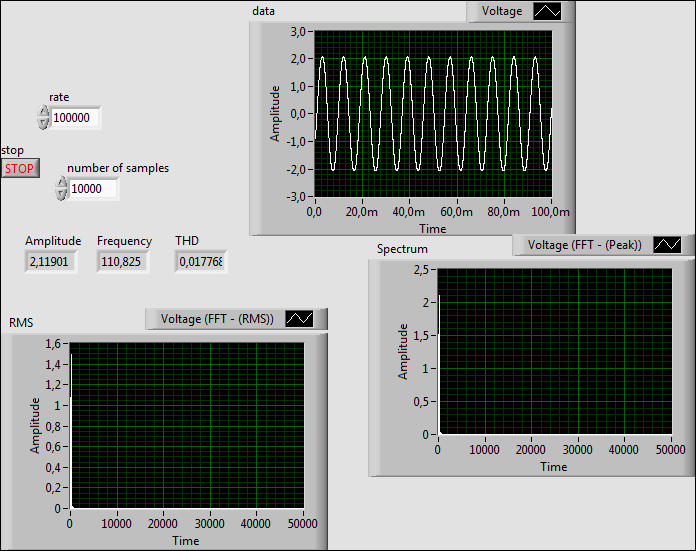
\includegraphics[width=\linewidth]{image/daa_vi}
	\caption{Передняя панель Data acquisition and analysis}\label{img:daa_vi}
\end{figure}

Код данной VI представлен на рис. \ref{img:daa_schema}.
Данные считываются до тех пор, пока не будет нажата кнопка остановки, при этом они постоянно выводятся на экран и обрабатываются.
Все представленные величины записываются в глобальные переменные для считывания из других программ.

\begin{figure}[H]
	\centering
	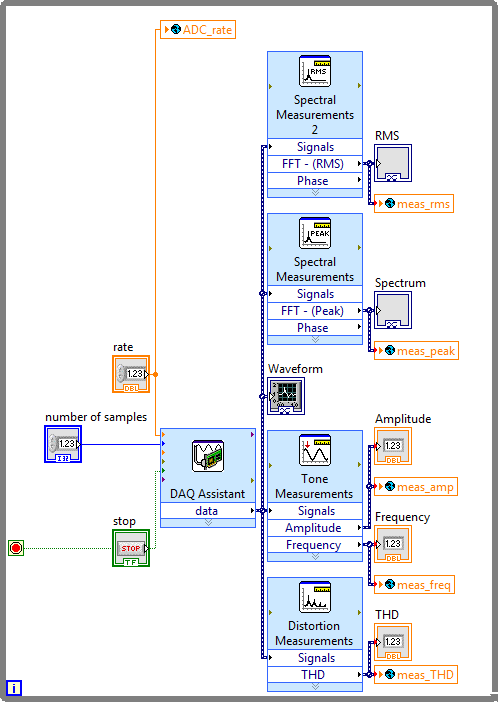
\includegraphics[width=\linewidth]{image/daa_schema}
	\caption{Блок-схема Data acquisition and analysis}\label{img:daa_schema}
\end{figure}

\subsection{ВП протоколирования результатов}

\label{subs:proto}

Данная VI (рис. \ref{img:daa_scaner_vi}) предназначена для обработки данных, полученных из предыдущей программы посредством глобальных переменных.
С помощью элементов управления можно задать число измерений и задержку между ними.
Стоит заметить, что данные замеры будут проводиться не с самого прибора, а с глобальных переменных (рис. \ref{img:daa_scaner_schema}), поэтому при низкой задержке может быть ситуация с дублированием данных при считывании, при большой -- потеря информации.
В любом случае, данную серьезную ошибку было бы здорово локализовать, например, с помощью синхросигналов на тех же глобальных переменных.
Тем не менее, это полностью не избавляет нас от данной проблемы и race condition, поэтому следовало бы использовать другие методы многопоточного проектирования связи между программами, если такие поддерживает LabView.

Значения полей <<Оператор>> и <<Путь к файлу протокола>> используются для сохранения отчёта.
На графике отображается текущее значение амплитуды. 
В матрицу выводится массив векторов с результатами обработки данных.

\begin{figure}[H]
	\centering
	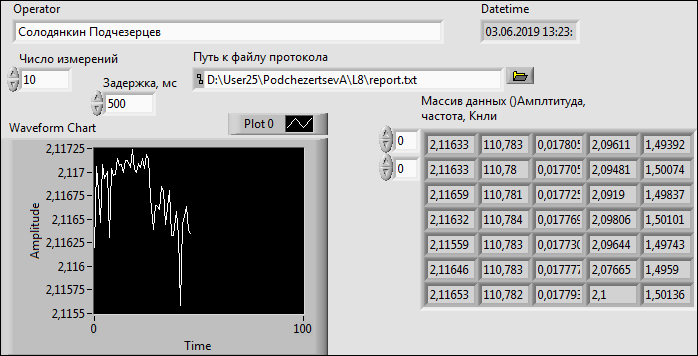
\includegraphics[width=\linewidth]{image/daa_scaner_vi}
	\caption{Передняя панель протоколирования для Data acquisition and analysis}\label{img:daa_scaner_vi}
\end{figure}

В структуре программы нет ничего сложного.
Сначала записывается форматированная строка из имени оператора прибора и текущей даты и времени, 
далее в следующую строку попадает информация с заголовками столбцов, 
после записывается массив всех измерений, который считывается в цикле.

\begin{figure}[H]
	\centering
	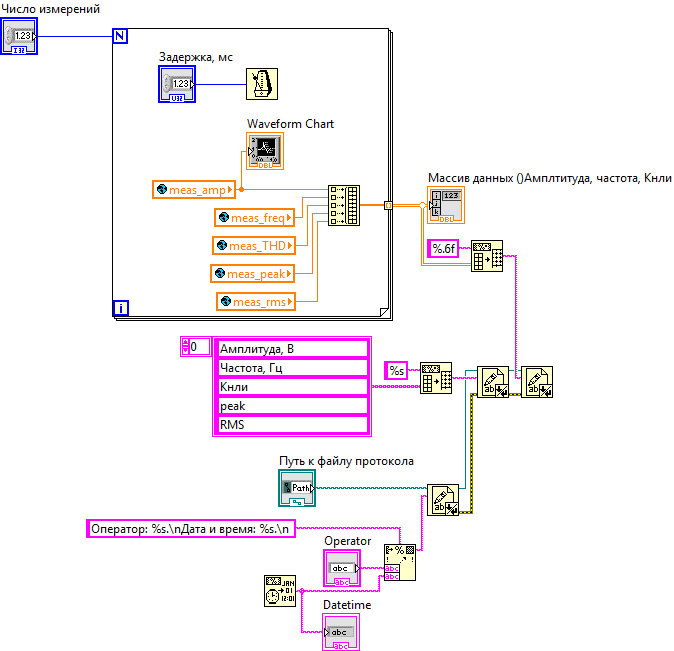
\includegraphics[width=\linewidth]{image/daa_scaner_schema}
	\caption{Блок-схема протоколирования для Data acquisition and analysis}\label{img:daa_scaner_schema}
\end{figure}

\subsection{ВП измерения частоты и периода}

VI на рис. \ref{img:dfm_freq_vi} и \ref{img:dfm_period_vi} представлены схемы для измерения периода или частоты.
С помощью элементов управления задается цель измерений, тип измерений, источник сигнала, минимальное и максимальное значение.
В единственное средство вывода будет отображено измеренное значение и тип измерений.

\begin{figure}[H]
	\centering
	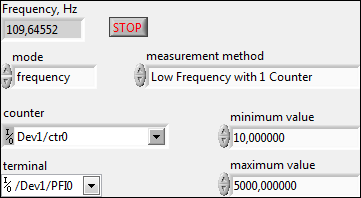
\includegraphics[width=\linewidth]{image/dfm_freq_vi}
	\caption{Передняя панель DAQ Frequency Meter с измерением частоты}\label{img:dfm_freq_vi}
\end{figure}

\begin{figure}[H]
	\centering
	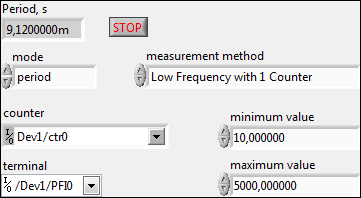
\includegraphics[width=\linewidth]{image/dfm_period_vi}
	\caption{Передняя панель DAQ Frequency Meter с измерением периода}\label{img:dfm_period_vi}
\end{figure}

Алгоритм обработки данных изображен на рис. \ref{img:dfm_schema}, шаг инициализации с частотой на рис. \ref{img:dfm_schema_init}, а период на рис. \ref{img:dfm_schema_period}. 
Случай чтения отображен на рис. \ref{img:dfm_schema_read}.
Алгоритм представлен в виде конечного автомата.
На шаге инициализации подготавливаются блоки считывания на основе введенных данных, затем начинается считывание, которое продолжается до тех пор, пока не будет произведена остановка или не произойдет ошибка.
Во время остановки обрабатываются возможные ошибки и программа завершается.

\begin{figure}[H]
	\centering
	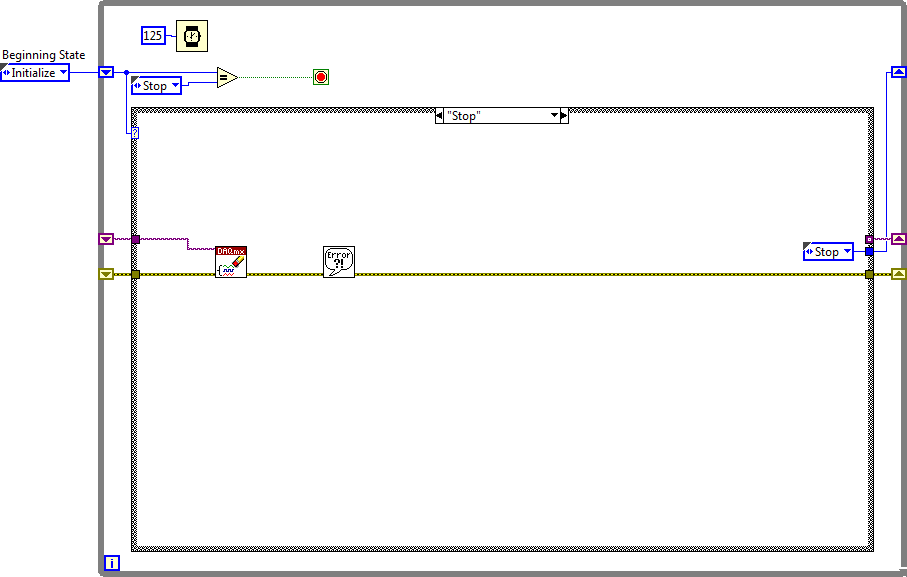
\includegraphics[width=\linewidth]{image/dfm_schema}
	\caption{Блок-схема DAQ Frequency Meter}\label{img:dfm_schema}
\end{figure}

\begin{figure}[H]
	\centering
	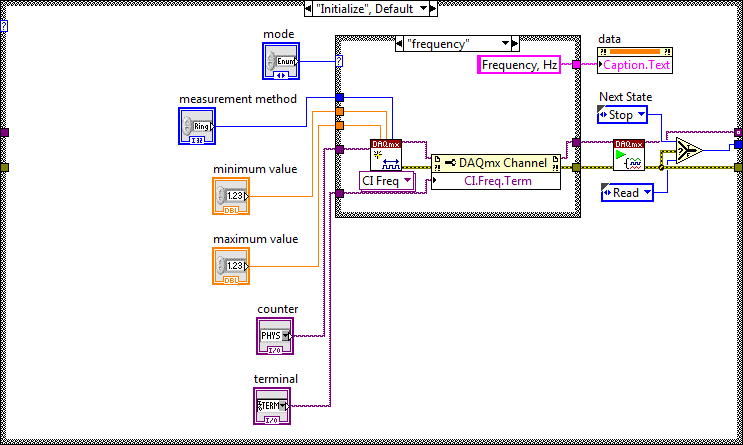
\includegraphics[width=\linewidth]{image/dfm_schema_init}
	\caption{Блок-схема DAQ Frequency Meter. Инициализация}\label{img:dfm_schema_init}
\end{figure}

\begin{figure}[H]
	\centering
	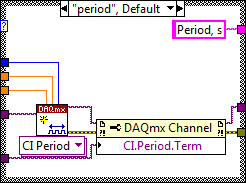
\includegraphics[width=0.7\linewidth]{image/dfm_schema_period}
	\caption{Блок-схема DAQ Frequency Meter. Обработка периода}\label{img:dfm_schema_period}
\end{figure}

\begin{figure}[H]
	\centering
	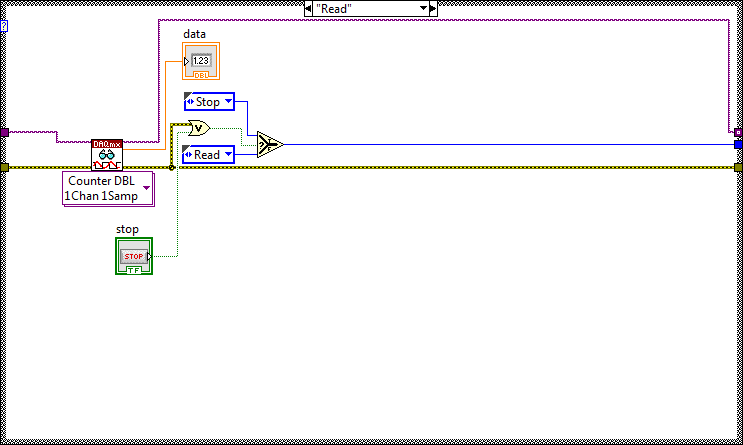
\includegraphics[width=\linewidth]{image/dfm_schema_read}
	\caption{Блок-схема DAQ Frequency Meter. Чтение}\label{img:dfm_schema_read}
\end{figure}

\subsection{ВП протоколирования результатов}

VI на рис. \ref{img:dfm_scaner_vi} и её блок-схема на рис. \ref{img:dfm_scanner_schema} изображены компоненты для считывания данных из глобальных переменных. Их принцип действия аналогичен тому, что описаны в разделе <<\nameref{subs:proto}>> на стр. \pageref{subs:proto}.

\begin{figure}[H]
	\centering
	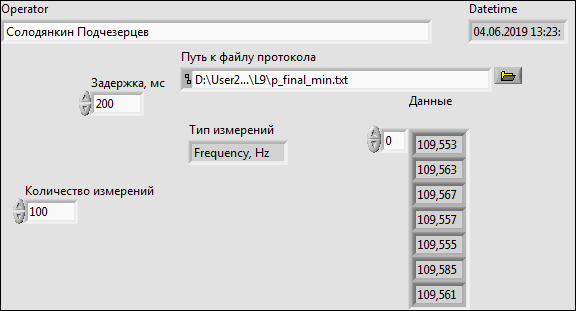
\includegraphics[width=\linewidth]{image/dfm_scaner_vi}
	\caption{Передняя панель протоколирования для DAQ Frequency Meter}\label{img:dfm_scaner_vi}
\end{figure}

\begin{figure}[H]
	\centering
	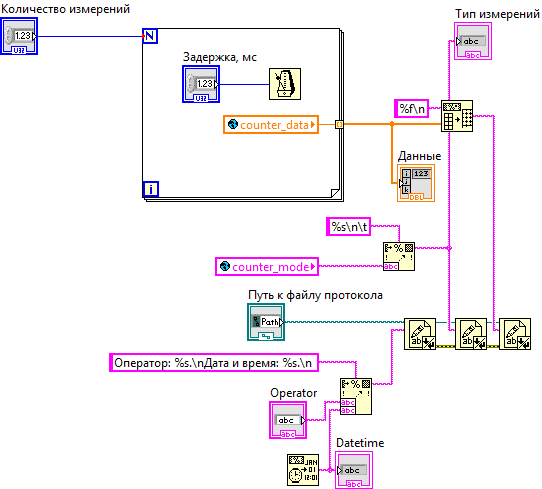
\includegraphics[width=\linewidth]{image/dfm_scanner_schema}
	\caption{Блок-схема протоколирования для DAQ Frequency Meter}\label{img:dfm_scanner_schema}
\end{figure}

\section{ПОРЯДОК ВЫПОЛНЕНИЯ РАБОТЫ}
\begin{enumerate}
	\item Проверка работоспособности оборудования в NI MAX. 
	\item Построение ВП для сбора и обработки данных на основе Express-VI.
	\item Построение ВП для формирования протокола. 
	\item Выполнение сбора и обработки данных. Получение измеренных значений амплитуды, частоты и коэффициента нелинейных искажений. Протоколирование измеренных значений (таблица \ref{tab:daa}).
	
	\item Построение ВП для сбора и обработки данных на основе DAQmx.
	\item Построение ВП для формирования протокола. 
	\item Выполнение сбора и обработки данных. Получение измеренных значений амплитуды, частоты. Протоколирование измеренных значений (таблицы \ref{tab:dfm_freq}, \ref{tab:dfm_scan_freq}, \ref{tab:dfm_scan_period}).
\end{enumerate}

\section{РЕЗУЛЬТАТЫ ИЗМЕРЕНИЙ И ВЫЧИСЛЕНИЙ}

\subsection{Результаты сбора данных}

\begin{table}[H]
	\centering
	\caption{Результаты Data acquisition and analysis}
	\label{tab:daa}
	\begin{tabular}{|l|l|l|l|l|}
		\hline
		Амплитуда, В & Частота, Гц & Кнли     & peak     & RMS      \\ \hline
		2,116329     & 110,782777  & 0,017806 & 2,096112 & 1,493919 \\ \hline
		2,116331     & 110,780089  & 0,017706 & 2,094815 & 1,500738 \\ \hline
		2,116586     & 110,780983  & 0,017725 & 2,091895 & 1,498371 \\ \hline
		2,116324     & 110,784142  & 0,017770 & 2,098058 & 1,501008 \\ \hline
		2,115589     & 110,783335  & 0,017731 & 2,096437 & 1,497431 \\ \hline
		2,116457     & 110,782877  & 0,017777 & 2,076650 & 1,495899 \\ \hline
		2,116525     & 110,782302  & 0,017794 & 2,100005 & 1,501362 \\ \hline
		2,116631     & 110,780192  & 0,017743 & 2,110060 & 1,491992 \\ \hline
		2,116387     & 110,783203  & 0,017763 & 2,106168 & 1,500619 \\ \hline
		2,116344     & 110,778854  & 0,017759 & 2,109736 & 1,501248 \\ \hline
	\end{tabular}
\end{table}

Амплитудное значение -- максимальное значение напряжения за 1 период.

Среднеквадратичное(действующее) значение -- эквивалент напряжения постоянного тока, при котором будет произведена такая же работа.

Для синусоидального сигнала:

$$ I = \frac{1}{\sqrt{2}} I_m $$

Где $I_m$ -- амплитудное значение, $I$ -- действующее.

\subsection{Результаты измерения частоты и периода}

\begin{longtable}[c]{|c|c|c|}
	\caption{Результаты измерения частоты в зависимости от позиции ручки регулятора}
	\label{tab:dfm_freq}\\
	\hline
	Frequency max, Hz & Frequency middle, Hz & Frequency min, Hz \\ \hline
	\endfirsthead
	%
	\endhead
	%
	9990.009990       & 205.689368           & 109.552874        \\ \hline
	9990.009990       & 205.689368           & 109.563226        \\ \hline
	9991.257650       & 205.688839           & 109.566828        \\ \hline
	9992.505621       & 205.686195           & 109.557224        \\ \hline
	9990.009990       & 205.690426           & 109.554824        \\ \hline
	9990.009990       & 205.670860           & 109.584838        \\ \hline
	9990.009990       & 205.680907           & 109.560975        \\ \hline
	9991.257650       & 205.687253           & 109.564577        \\ \hline
	9990.009990       & 205.703648           & 109.556774        \\ \hline
	9990.009990       & 205.690426           & 109.575682        \\ \hline
	9991.257650       & 205.683551           & 109.563826        \\ \hline
	9990.009990       & 205.684608           & 109.555124        \\ \hline
	9991.257650       & 205.674032           & 109.555874        \\ \hline
	9990.009990       & 205.683022           & 109.561276        \\ \hline
	9988.762642       & 205.693599           & 109.555424        \\ \hline
	9988.762642       & 205.667159           & 109.575382        \\ \hline
	9990.009990       & 205.687781           & 109.557825        \\ \hline
	9990.009990       & 205.654998           & 109.569829        \\ \hline
	9990.009990       & 205.661871           & 109.563226        \\ \hline
	9990.009990       & 205.707350           & 109.538923        \\ \hline
	9990.009990       & 205.688310           & 109.566677        \\ \hline
	9990.009990       & 205.680378           & 109.550323        \\ \hline
	9990.009990       & 205.659756           & 109.571330        \\ \hline
	9990.009990       & 205.681435           & 109.530825        \\ \hline
	9988.762642       & 205.695714           & 109.552574        \\ \hline
	9991.257650       & 205.679320           & 109.572530        \\ \hline
	9990.009990       & 205.692541           & 109.562776        \\ \hline
	9991.257650       & 205.695185           & 109.582286        \\ \hline
	9991.257650       & 205.677734           & 109.544773        \\ \hline
	9988.762642       & 205.690954           & 109.558725        \\ \hline
	9988.762642       & 205.696243           & 109.522577        \\ \hline
	9988.762642       & 205.650240           & 109.521978        \\ \hline
	9990.009990       & 205.619583           & 109.558575        \\ \hline
	9988.762642       & 205.696243           & 109.541323        \\ \hline
	9990.009990       & 205.680907           & 109.554224        \\ \hline
	9988.762642       & 205.679849           & 109.577483        \\ \hline
	9990.009990       & 205.698359           & 109.564727        \\ \hline
	9988.762642       & 205.688310           & 109.544323        \\ \hline
	9990.009990       & 205.660285           & 109.528425        \\ \hline
	9990.009990       & 205.686724           & 109.548973        \\ \hline
	9990.009990       & 205.725865           & 109.545523        \\ \hline
	9988.762642       & 205.684080           & 109.557525        \\ \hline
	9988.762642       & 205.676147           & 109.551523        \\ \hline
	9988.762642       & 205.710524           & 109.546723        \\ \hline
	9991.257650       & 205.717930           & 109.555874        \\ \hline
	9990.009990       & 205.649712           & 109.515531        \\ \hline
	9990.009990       & 205.669802           & 109.526926        \\ \hline
	9990.009990       & 205.682493           & 109.548673        \\ \hline
	9987.515605       & 205.669274           & 109.525576        \\ \hline
	9988.762642       & 205.671917           & 109.536674        \\ \hline
	9990.009990       & 205.665044           & 109.565477        \\ \hline
	9990.009990       & 205.669274           & 109.573281        \\ \hline
	9988.762642       & 205.702590           & 109.556024        \\ \hline
	9990.009990       & 205.638082           & 109.547623        \\ \hline
	9990.009990       & 205.686724           & 109.550923        \\ \hline
	9990.009990       & 205.711582           & 109.565027        \\ \hline
	9988.762642       & 205.665044           & 109.551974        \\ \hline
	9987.515605       & 205.679320           & 109.539373        \\ \hline
	9988.762642       & 205.711582           & 109.537273        \\ \hline
	9988.762642       & 205.681435           & 109.542823        \\ \hline
	9988.762642       & 205.660814           & 109.530375        \\ \hline
	9988.762642       & 205.676676           & 109.548523        \\ \hline
	9988.762642       & 205.677205           & 109.557224        \\ \hline
	9988.762642       & 205.674032           & 109.542523        \\ \hline
	9990.009990       & 205.673504           & 109.536974        \\ \hline
	9990.009990       & 205.690426           & 109.542073        \\ \hline
	9990.009990       & 205.698888           & 109.533524        \\ \hline
	9990.009990       & 205.675619           & 109.553024        \\ \hline
	9988.762642       & 205.700474           & 109.573431        \\ \hline
	9987.515605       & 205.704177           & 109.489601        \\ \hline
	9990.009990       & 205.692541           & 109.535474        \\ \hline
	9990.009990       & 205.689897           & 109.533374        \\ \hline
	9990.009990       & 205.684608           & 109.528875        \\ \hline
	9988.762642       & 205.713169           & 109.531724        \\ \hline
	9988.762642       & 205.659228           & 109.535624        \\ \hline
	9987.515605       & 205.724807           & 109.548523        \\ \hline
	9990.009990       & 205.714227           & 109.530375        \\ \hline
	9988.762642       & 205.706821           & 109.555424        \\ \hline
	9988.762642       & 205.709995           & 109.536524        \\ \hline
	9988.762642       & 205.709466           & 109.543273        \\ \hline
	9988.762642       & 205.706293           & 109.544923        \\ \hline
	9988.762642       & 205.697301           & 109.541773        \\ \hline
	9990.009990       & 205.663986           & 109.541923        \\ \hline
	9988.762642       & 205.717401           & 109.554074        \\ \hline
	9988.762642       & 205.690954           & 109.550623        \\ \hline
	9987.515605       & 205.696772           & 109.541773        \\ \hline
	9988.762642       & 205.709995           & 109.529025        \\ \hline
	9988.762642       & 205.706293           & 109.541173        \\ \hline
	9988.762642       & 205.722162           & 109.530225        \\ \hline
	9988.762642       & 205.674032           & 109.517180        \\ \hline
	9987.515605       & 205.704706           & 109.557975        \\ \hline
	9987.515605       & 205.701532           & 109.537573        \\ \hline
	9987.515605       & 205.686724           & 109.537273        \\ \hline
	9990.009990       & 205.702590           & 109.544023        \\ \hline
	9990.009990       & 205.712111           & 109.537723        \\ \hline
	9988.762642       & 205.691483           & 109.548973        \\ \hline
	9988.762642       & 205.702590           & 109.541623        \\ \hline
	9988.762642       & 205.712111           & 109.530975        \\ \hline
	9988.762642       & 205.716343           & 109.528425        \\ \hline
	9988.762642       & 205.697301           & 109.541923        \\ \hline
\end{longtable}

\begin{table}[H]
	\centering
	\caption{Результат измерения частоты}
	\label{tab:dfm_scan_freq}
	\begin{tabular}{|c|}
		\hline
		Frequency, Hz \\ \hline
		 109.557224   \\ \hline
		 109.563976   \\ \hline
		 109.560375   \\ \hline
		 109.546573   \\ \hline
		 109.550623   \\ \hline
		 109.550173   \\ \hline
		 109.572680   \\ \hline
		 109.540273   \\ \hline
		 109.559625   \\ \hline
		 109.566227   \\ \hline
	\end{tabular}
\end{table}

\begin{table}[H]
	\centering
	\caption{Результат измерения периода}
	\label{tab:dfm_scan_period}
	\begin{tabular}{|c|}
		\hline
		Period, s \\ \hline
		0.009130  \\ \hline
		0.009130  \\ \hline
		0.009120  \\ \hline
		0.009120  \\ \hline
		0.009130  \\ \hline
		0.009120  \\ \hline
		0.009130  \\ \hline
		0.009130  \\ \hline
		0.009130  \\ \hline
		0.009130  \\ \hline
	\end{tabular}
\end{table}

\section{ВЫВОДЫ ПО РАБОТЕ}

В ходе работы были получены следующие результаты:

\begin{itemize} 
	\item ПО NI-MAX и инструменты DAQmx позволяют проводить измерения серий данных и проводить их статистическую и частотную обработку.
	\item В данных работах были использованы алгоритмические структуры циклы while, for, оператор множественного выбора switch/case, условный оператор, тернарный оператор (select), константы.
	Для передачи данных от одной итерации цикла к последующим использовались сдвиговые регистры.
	Связь между программами была основана на глобальных переменных. 
	Недостатки данного подхода были описаны в разделе <<\nameref{subs:proto}>> на стр. \pageref{subs:proto}.
	\item Для реализации паттерна конечного автомата использовалась константа со списком всех состояний, цикл while, который останавливался при шаге завершения работы, структура case, в которой были определены действия для каждого случая и следующая итерация в зависимости от ситуации.
\end{itemize}

\end{document} % конец документа